\documentclass[11pt,a4paper]{article}
\usepackage[utf8]{inputenc}
\usepackage[left=2.3cm,right=2.3cm,top=2.5cm,bottom=2.5cm]{geometry}
\usepackage{amsmath,amssymb,amsfonts}
\usepackage{array}
\usepackage{enumitem}
\usepackage{fancyhdr}
\setlength{\headheight}{14pt}
\usepackage{hyperref}
\usepackage{tikz}
\usetikzlibrary{arrows.meta, positioning, calc, shapes.geometric}

\tikzset{
    block/.style = {draw, rectangle, minimum height=1cm, minimum width=1.5cm, align=center, thick, fill=blue!5},
    sum/.style = {draw, circle, node distance=1.5cm, minimum size=6mm, thick, fill=gray!10},
    input/.style = {coordinate},
    output/.style = {coordinate},
    sfgnode/.style={circle, fill=blue!15, draw=blue!70, thick, minimum size=7mm, inner sep=0pt, font=\small\bfseries},
    sfgarrow/.style={-{Latex[length=2.5mm,width=1.5mm]}, thick, draw=blue!80!black},
    sfgloop/.style={-{Latex[length=2.5mm,width=1.5mm]}, thick, draw=red!75!black}
}

\pagestyle{fancy}
\fancyhf{}
\rhead{\textbf{MA4171 Teori Kontrol Linear}}
\lhead{\textbf{Latihan Matematis: Pemodelan Ruang Keadaan}}
\rfoot{Halaman \thepage}

\hypersetup{
    colorlinks=true,
    linkcolor=blue,
    urlcolor=cyan
}

\setlength{\parindent}{0pt}
\setlength{\parskip}{5pt}

\begin{document}

\begin{center}
    {\Large \textbf{LEMBAR LATIHAN DAN PEMBAHASAN MATEMATIS}}\\[4pt]
    {\large \textbf{TOPIK 02: PEMODELAN RUANG KEADAAN \& MATRIKS FUNDAMENTAL}}\\[4pt]
    \textbf{Mata Kuliah:} MA4171 Teori Kontrol Linear --- FMIPA ITB
\end{center}
\hrule
\vspace{10pt}

% =========================================================================
% SOAL 1
% =========================================================================
\textbf{\large No. 1}

\textbf{Soal:}  
Diberikan persamaan diferensial linear invarian waktu (LTI) orde-3 dengan turunan pada fungsi masukan:
$$\dddot{y}(t) + 6\ddot{y}(t) + 11\dot{y}(t) + 6y(t) = 4\dot{u}(t) + 2u(t)$$
dengan seluruh kondisi awal diasumsikan bernilai nol pada $t = 0$.
\begin{enumerate}[label=(\alph*)]
    \item Tentukan fungsi transfer $G(s) = \frac{Y(s)}{U(s)}$ sistem tersebut.
    \item Tentukan representasi ruang keadaan dalam Bentuk Kanonik Keterkontrolan (\textit{Controllable Canonical Form}, CCF) menggunakan metode variabel perantara $Z(s)$.
    \item Tentukan representasi ruang keadaan dalam Bentuk Kanonik Keterobservasian (\textit{Observable Canonical Form}, OCF).
\end{enumerate}

\textbf{Penyelesaian:}

\textbf{(a) Penentuan Fungsi Transfer}

Diberikan persamaan diferensial sistem:
$$\dddot{y}(t) + 6\ddot{y}(t) + 11\dot{y}(t) + 6y(t) = 4\dot{u}(t) + 2u(t)$$

Transformasi Laplace diterapkan secara linear pada kedua ruas persamaan diferensial:
$$\mathcal{L}\{\dddot{y}(t)\} + 6\mathcal{L}\{\ddot{y}(t)\} + 11\mathcal{L}\{\dot{y}(t)\} + 6\mathcal{L}\{y(t)\} = 4\mathcal{L}\{\dot{u}(t)\} + 2\mathcal{L}\{u(t)\}$$

Berdasarkan sifat transformasi Laplace untuk turunan waktu:
\begin{align*}
    \mathcal{L}\{\dddot{y}(t)\} &= s^3 Y(s) - s^2 y(0) - s \dot{y}(0) - \ddot{y}(0) \\
    \mathcal{L}\{\ddot{y}(t)\} &= s^2 Y(s) - s y(0) - \dot{y}(0) \\
    \mathcal{L}\{\dot{y}(t)\} &= s Y(s) - y(0) \\
    \mathcal{L}\{y(t)\} &= Y(s)
\end{align*}
serta untuk fungsi masukan:
\begin{align*}
    \mathcal{L}\{\dot{u}(t)\} &= s U(s) - u(0) \\
    \mathcal{L}\{u(t)\} &= U(s)
\end{align*}

Fungsi transfer sistem didefinisikan pada kondisi awal nol ($y(0) = 0$, $\dot{y}(0) = 0$, $\ddot{y}(0) = 0$, dan $u(0) = 0$), sehingga seluruh suku kondisi awal lenyap. Substitusi hasil transformasi ke dalam persamaan menghasilkan:
$$s^3 Y(s) + 6s^2 Y(s) + 11s Y(s) + 6Y(s) = 4s U(s) + 2U(s)$$

Variabel $Y(s)$ pada ruas kiri dan $U(s)$ pada ruas kanan difaktorkan ke luar:
$$(s^3 + 6s^2 + 11s + 6) Y(s) = (4s + 2) U(s)$$

Dengan membagi kedua ruas dengan polinomial karakteristik $(s^3 + 6s^2 + 11s + 6)$ dan membagi dengan $U(s)$, diperoleh fungsi transfer sistem:
$$G(s) = \frac{Y(s)}{U(s)} = \frac{4s + 2}{s^3 + 6s^2 + 11s + 6}$$

\textbf{(b) Konstruksi Bentuk Kanonik Keterkontrolan (CCF)}

Untuk memisahkan dinamika masukan dan keluaran secara sistematis tanpa melibatkan diferensiasi langsung dari sinyal kontrol $u(t)$, diperkenalkan suatu variabel perantara skalar $Z(s)$ sedemikian rupa sehingga:
$$Z(s) = \frac{U(s)}{s^3 + 6s^2 + 11s + 6} \implies (s^3 + 6s^2 + 11s + 6) Z(s) = U(s)$$
dan persamaan sinyal keluaran dinyatakan oleh pembilang fungsi transfer:
$$Y(s) = (4s + 2) Z(s) = 4s Z(s) + 2 Z(s)$$

Dalam domain waktu, persamaan diferensial untuk variabel perantara $z(t)$ berbentuk:
$$\dddot{z}(t) + 6\ddot{z}(t) + 11\dot{z}(t) + 6z(t) = u(t) \implies \dddot{z}(t) = -6z(t) - 11\dot{z}(t) - 6\ddot{z}(t) + u(t)$$

Variabel-variabel keadaan didefinisikan sebagai turunan berurutan dari variabel perantara:
$$x_1(t) = z(t), \quad x_2(t) = \dot{z}(t), \quad x_3(t) = \ddot{z}(t)$$

Diferensiasi terhadap waktu untuk masing-masing variabel keadaan menghasilkan persamaan ruang keadaan:
$$\dot{x}_1(t) = x_2(t)$$
$$\dot{x}_2(t) = x_3(t)$$
$$\dot{x}_3(t) = \dddot{z}(t) = -6x_1(t) - 11x_2(t) - 6x_3(t) + u(t)$$

Persamaan keluaran diperoleh melalui invers transformasi Laplace dari ekspresi $Y(s)$:
$$y(t) = 2z(t) + 4\dot{z}(t) = 2x_1(t) + 4x_2(t) + 0x_3(t)$$

Dalam notasi matriks standar $\dot{\mathbf{x}} = A\mathbf{x} + B u$ dan $y = C\mathbf{x} + D u$:
$$A_{ccf} = \begin{bmatrix} 0 & 1 & 0 \\ 0 & 0 & 1 \\ -6 & -11 & -6 \end{bmatrix}, \quad B_{ccf} = \begin{bmatrix} 0 \\ 0 \\ 1 \end{bmatrix}$$
$$C_{ccf} = \begin{bmatrix} 2 & 4 & 0 \end{bmatrix}, \quad D_{ccf} = 0$$

\textbf{(c) Konstruksi Bentuk Kanonik Keterobservasian (OCF)}

Bentuk kanonik keterobservasian merupakan dual dari bentuk kanonik keterkontrolan. Koefisien-koefisien pembilang ditempatkan pada matriks masukan $B$, sedangkan koefisien penyebut ditempatkan pada kolom terakhir matriks sistem:
$$A_{ocf} = A_{ccf}^T = \begin{bmatrix} 0 & 0 & -6 \\ 1 & 0 & -11 \\ 0 & 1 & -6 \end{bmatrix}, \quad B_{ocf} = C_{ccf}^T = \begin{bmatrix} 2 \\ 4 \\ 0 \end{bmatrix}$$
$$C_{ocf} = B_{ccf}^T = \begin{bmatrix} 0 & 0 & 1 \end{bmatrix}, \quad D_{ocf} = 0$$

\vspace{12pt}
\hrule
\vspace{10pt}

% =========================================================================
% SOAL 2
% =========================================================================
\textbf{\large No. 2}

\textbf{Soal:}  
Diberikan fungsi transfer sistem kontinu berikut:
$$G(s) = \frac{3s + 7}{(s+1)(s+2)(s+3)}$$
\begin{enumerate}[label=(\alph*)]
    \item Uraikan fungsi transfer $G(s)$ ke dalam bentuk penjumlahan pecahan parsial.
    \item Tentukan persamaan ruang keadaan dalam Bentuk Kanonik Diagonal (\textit{Diagonal Canonical Form}, DCF).
    \item Tuliskan persamaan diferensial untuk setiap variabel keadaan hasil dekomposisi tersebut dan jelaskan mengapa bentuk ini dinamakan ter-dekopel (\textit{decoupled}).
\end{enumerate}

\textbf{Penyelesaian:}

\textbf{(a) Dekomposisi Pecahan Parsial}

Penyebut fungsi transfer memiliki tiga kutub riil yang saling berbeda, yaitu $s = -1$, $s = -2$, dan $s = -3$. Fungsi transfer dapat diuraikan menjadi:
$$G(s) = \frac{R_1}{s+1} + \frac{R_2}{s+2} + \frac{R_3}{s+3}$$

Masing-masing residu dihitung menggunakan metode penutupan (\textit{Heaviside cover-up method}):
Residu pertama pada kutub $s = -1$:
$$R_1 = \lim_{s \to -1} (s+1) G(s) = \left. \frac{3s + 7}{(s+2)(s+3)} \right|_{s=-1} = \frac{3(-1) + 7}{(-1+2)(-1+3)} = \frac{4}{(1)(2)} = 2$$

Residu kedua pada kutub $s = -2$:
$$R_2 = \lim_{s \to -2} (s+2) G(s) = \left. \frac{3s + 7}{(s+1)(s+3)} \right|_{s=-2} = \frac{3(-2) + 7}{(-2+1)(-2+3)} = \frac{1}{(-1)(1)} = -1$$

Residu ketiga pada kutub $s = -3$:
$$R_3 = \lim_{s \to -3} (s+3) G(s) = \left. \frac{3s + 7}{(s+1)(s+2)} \right|_{s=-3} = \frac{3(-3) + 7}{(-3+1)(-3+2)} = \frac{-2}{(-2)(-1)} = -1$$

Dengan demikian, bentuk pecahan parsial fungsi transfer adalah:
$$G(s) = \frac{2}{s+1} - \frac{1}{s+2} - \frac{1}{s+3}$$

\textbf{(b) Penyusunan Bentuk Kanonik Diagonal (DCF)}

Didefinisikan variabel keadaan dalam domain Laplace untuk masing-masing moda eigen sebagai:
$$X_1(s) = \frac{1}{s+1} U(s), \quad X_2(s) = \frac{1}{s+2} U(s), \quad X_3(s) = \frac{1}{s+3} U(s)$$

Sinyal keluaran $Y(s) = G(s) U(s)$ dinyatakan sebagai kombinasi linear dari variabel keadaan:
$$Y(s) = 2 X_1(s) - X_2(s) - X_3(s)$$

Transformasi balik ke domain waktu menghasilkan sistem matriks diagonal:
$$A_{diag} = \begin{bmatrix} -1 & 0 & 0 \\ 0 & -2 & 0 \\ 0 & 0 & -3 \end{bmatrix}, \quad B_{diag} = \begin{bmatrix} 1 \\ 1 \\ 1 \end{bmatrix}$$
$$C_{diag} = \begin{bmatrix} 2 & -1 & -1 \end{bmatrix}, \quad D_{diag} = 0$$

\textbf{(c) Karakteristik Ter-dekopel}

Persamaan diferensial untuk masing-masing variabel keadaan adalah:
$$\dot{x}_1(t) = -x_1(t) + u(t)$$
$$\dot{x}_2(t) = -2x_2(t) + u(t)$$
$$\dot{x}_3(t) = -3x_3(t) + u(t)$$

Sistem ini disebut ter-dekopel (\textit{decoupled}) karena laju perubahan dari setiap variabel keadaan $\dot{x}_i(t)$ hanya bergantung secara eksklusif pada dirinya sendiri $x_i(t)$ dan masukan luar $u(t)$, tanpa adanya interaksi atau ketergantungan silang dengan variabel keadaan lainnya ($x_j(t)$ untuk $j \ne i$).

\vspace{12pt}
\hrule
\vspace{10pt}

% =========================================================================
% SOAL 3
% =========================================================================
\textbf{\large No. 3}

\textbf{Soal:}  
Diberikan fungsi transfer dengan kutub berulang (multiplisitas 3):
$$G(s) = \frac{2s^2 + 5s + 4}{(s+1)^3}$$
\begin{enumerate}[label=(\alph*)]
    \item Uraikan fungsi transfer $G(s)$ ke dalam basis pecahan parsial dengan penyebut perpangkatan $(s+1)$.
    \item Susun representasi ruang keadaan sistem dalam Bentuk Kanonik Jordan (\textit{Jordan Canonical Form}, JCF) di mana matriks sistem memuat satu blok Jordan tunggal.
    \item Verifikasi kebenaran matriks ruang keadaan yang diperoleh dengan menghitung kembali fungsi transfer $G(s) = C(sI - A)^{-1} B$.
\end{enumerate}

\textbf{Penyelesaian:}

\textbf{(a) Ekspansi Pecahan Parsial Basis $(s+1)$}

Polinomial pembilang dinyatakan dalam variabel pergeseran $p = s + 1 \implies s = p - 1$:
$$2s^2 + 5s + 4 = 2(p - 1)^2 + 5(p - 1) + 4 = 2(p^2 - 2p + 1) + 5p - 5 + 4 = 2p^2 + p + 1$$

Dengan mengembalikan substitusi $p = s + 1$, diperoleh bentuk pembilang:
$$2s^2 + 5s + 4 = 2(s+1)^2 + (s+1) + 1$$

Pembagian setiap suku dengan penyebut $(s+1)^3$ menghasilkan ekspansi pecahan parsial:
$$G(s) = \frac{2(s+1)^2}{(s+1)^3} + \frac{s+1}{(s+1)^3} + \frac{1}{(s+1)^3} = \frac{2}{s+1} + \frac{1}{(s+1)^2} + \frac{1}{(s+1)^3}$$

\textbf{(b) Penyusunan Bentuk Kanonik Jordan (JCF)}

Untuk membentuk satu blok Jordan berordo $3 \times 3$, rantai variabel keadaan didefinisikan secara bertingkat:
$$X_3(s) = \frac{1}{s+1} U(s) \implies (s+1) X_3(s) = U(s)$$
$$X_2(s) = \frac{1}{s+1} X_3(s) = \frac{1}{(s+1)^2} U(s) \implies (s+1) X_2(s) = X_3(s)$$
$$X_1(s) = \frac{1}{s+1} X_2(s) = \frac{1}{(s+1)^3} U(s) \implies (s+1) X_1(s) = X_2(s)$$

Dalam domain waktu, sistem diferensial bertingkat tersebut menjadi:
$$\dot{x}_1(t) = -x_1(t) + x_2(t)$$
$$\dot{x}_2(t) = -x_2(t) + x_3(t)$$
$$\dot{x}_3(t) = -x_3(t) + u(t)$$

Persamaan keluaran dinyatakan sesuai ekspansi pecahan parsial:
$$Y(s) = X_1(s) + X_2(s) + 2X_3(s) \implies y(t) = x_1(t) + x_2(t) + 2x_3(t)$$

Matriks ruang keadaan dalam bentuk blok Jordan adalah:
$$A_J = \begin{bmatrix} -1 & 1 & 0 \\ 0 & -1 & 1 \\ 0 & 0 & -1 \end{bmatrix}, \quad B_J = \begin{bmatrix} 0 \\ 0 \\ 1 \end{bmatrix}$$
$$C_J = \begin{bmatrix} 1 & 1 & 2 \end{bmatrix}, \quad D_J = 0$$

\textbf{(c) Verifikasi Fungsi Transfer}

Matriks karakteristik $(sI - A_J)$ adalah matriks segitiga atas:
$$sI - A_J = \begin{bmatrix} s+1 & -1 & 0 \\ 0 & s+1 & -1 \\ 0 & 0 & s+1 \end{bmatrix}$$

Invers matriks segitiga atas dihitung secara langsung:
$$(sI - A_J)^{-1} = \begin{bmatrix} \frac{1}{s+1} & \frac{1}{(s+1)^2} & \frac{1}{(s+1)^3} \\ 0 & \frac{1}{s+1} & \frac{1}{(s+1)^2} \\ 0 & 0 & \frac{1}{s+1} \end{bmatrix}$$

Perkalian resolven dengan vektor masukan $B_J$ mengekstraksi kolom ketiga:
$$(sI - A_J)^{-1} B_J = \begin{bmatrix} \frac{1}{(s+1)^3} \\ \frac{1}{(s+1)^2} \\ \frac{1}{s+1} \end{bmatrix}$$

Perkalian dengan vektor baris keluaran $C_J$ menghasilkan:
$$G(s) = C_J (sI - A_J)^{-1} B_J = \begin{bmatrix} 1 & 1 & 2 \end{bmatrix} \begin{bmatrix} \frac{1}{(s+1)^3} \\ \frac{1}{(s+1)^2} \\ \frac{1}{s+1} \end{bmatrix} = \frac{1}{(s+1)^3} + \frac{1}{(s+1)^2} + \frac{2}{s+1} = \frac{2s^2 + 5s + 4}{(s+1)^3}$$
Hasil verifikasi tepat identik dengan fungsi transfer awal.

\vspace{12pt}
\hrule
\vspace{10pt}

% =========================================================================
% SOAL 4
% =========================================================================
\textbf{\large No. 4}

\textbf{Soal:}  
Suatu sistem dinamik linear didefinisikan oleh matriks ruang keadaan:
$$A = \begin{bmatrix} 0 & 1 & 0 \\ 0 & 0 & 1 \\ -6 & -11 & -6 \end{bmatrix}, \quad B = \begin{bmatrix} 0 \\ 1 \\ 2 \end{bmatrix}, \quad C = \begin{bmatrix} 1 & 1 & 0 \end{bmatrix}, \quad D = 0$$
\begin{enumerate}[label=(\alph*)]
    \item Hitung determinan $\det(sI - A)$ dan matriks adjoin $\operatorname{adj}(sI - A)$.
    \item Tentukan fungsi transfer $G(s) = C(sI - A)^{-1} B + D$.
    \item Identifikasi apakah terdapat pembatalan faktor persekutuan (\textit{pole-zero cancellation}) pada fungsi transfer yang dihasilkan.
\end{enumerate}

\textbf{Penyelesaian:}

\textbf{(a) Perhitungan Determinan dan Matriks Adjoin}

Dibentuk matriks $(sI - A)$:
$$sI - A = \begin{bmatrix} s & -1 & 0 \\ 0 & s & -1 \\ 6 & 11 & s+6 \end{bmatrix}$$

Determinan dihitung melalui ekspansi baris pertama:
\begin{align*}
    \det(sI - A) &= s [s(s+6) - (-1)(11)] - (-1) [0(s+6) - (-1)(6)] + 0 \\
    &= s [s^2 + 6s + 11] + [6] \\
    &= s^3 + 6s^2 + 11s + 6 = (s+1)(s+2)(s+3)
\end{align*}

Matriks kofaktor $K_{ij}$ dihitung untuk setiap elemen matriks $(sI - A)$, kemudian ditransposisikan untuk memperoleh matriks adjoin:
$$\operatorname{adj}(sI - A) = \begin{bmatrix} s^2+6s+11 & s+6 & 1 \\ -6 & s(s+6) & s \\ -6s & -(11s+6) & s^2 \end{bmatrix}$$

\textbf{(b) Penentuan Fungsi Transfer}

Dihitung perkalian vektor baris $C$ dengan matriks adjoin:
$$C \operatorname{adj}(sI - A) = \begin{bmatrix} 1 & 1 & 0 \end{bmatrix} \begin{bmatrix} s^2+6s+11 & s+6 & 1 \\ -6 & s^2+6s & s \\ -6s & -(11s+6) & s^2 \end{bmatrix} = \begin{bmatrix} s^2+6s+5 & s^2+7s+6 & s+1 \end{bmatrix}$$

Perhatikan bahwa setiap elemen vektor baris tersebut memiliki faktor persekutuan $(s+1)$:
$$C \operatorname{adj}(sI - A) = (s+1) \begin{bmatrix} s+5 & s+6 & 1 \end{bmatrix}$$

Selanjutnya dikalikan dengan vektor kolom masukan $B$:
\begin{align*}
    C \operatorname{adj}(sI - A) B &= (s+1) \begin{bmatrix} s+5 & s+6 & 1 \end{bmatrix} \begin{bmatrix} 0 \\ 1 \\ 2 \end{bmatrix} \\
    &= (s+1) [0(s+5) + 1(s+6) + 2(1)] \\
    &= (s+1) [s + 8]
\end{align*}

Fungsi transfer sistem adalah rasio antara hasil kali skalar tersebut dengan determinan:
$$G(s) = \frac{C \operatorname{adj}(sI - A) B}{\det(sI - A)} = \frac{(s+1)(s+8)}{(s+1)(s+2)(s+3)}$$

\textbf{(c) Pembatalan Faktor Persekutuan (\textit{Pole-Zero Cancellation})}

Faktor $(s+1)$ muncul baik pada pembilang maupun penyebut. Setelah dilakukan pembatalan faktor persekutuan tersebut:
$$G(s) = \frac{s + 8}{(s+2)(s+3)} = \frac{s + 8}{s^2 + 5s + 6}$$

Pembatalan faktor $(s+1)$ ini menunjukkan bahwa moda dinamis yang berkorespondensi dengan nilai eigen $\lambda = -1$ tidak teramati secara menyeluruh pada hubungan masukan-keluaran sistem.

\vspace{12pt}
\hrule
\vspace{10pt}

% =========================================================================
% SOAL 5
% =========================================================================
\textbf{\large No. 5}

\textbf{Soal:}  
Diberikan matriks dinamika sistem LTI kontinu orde-2:
$$A = \begin{bmatrix} 0 & 1 \\ -2 & -3 \end{bmatrix}$$
\begin{enumerate}[label=(\alph*)]
    \item Tentukan matriks resolven $(sI - A)^{-1}$ dalam domain frekuensi kompleks $s$.
    \item Dengan menerapkan invers transformasi Laplace elemen demi elemen, tentukan matriks fundamental (matriks transisi keadaan) $\Phi(t) = e^{At}$.
    \item Verifikasi sifat-sifat identitas matriks fundamental: $\Phi(0) = I$ dan $\left.\frac{d}{dt}\Phi(t)\right|_{t=0} = A$.
\end{enumerate}

\textbf{Penyelesaian:}

\textbf{(a) Penentuan Matriks Resolven}

Matriks karakteristik $(sI - A)$ adalah:
$$sI - A = \begin{bmatrix} s & -1 \\ 2 & s+3 \end{bmatrix}$$

Determinan matriks karakteristik:
$$\det(sI - A) = s(s+3) - (-1)(2) = s^2 + 3s + 2 = (s+1)(s+2)$$

Matriks invers dihitung melalui rumus invers matriks $2 \times 2$:
$$(sI - A)^{-1} = \frac{1}{(s+1)(s+2)} \begin{bmatrix} s+3 & 1 \\ -2 & s \end{bmatrix} = \begin{bmatrix} \frac{s+3}{(s+1)(s+2)} & \frac{1}{(s+1)(s+2)} \\ \frac{-2}{(s+1)(s+2)} & \frac{s}{(s+1)(s+2)} \end{bmatrix}$$

\textbf{(b) Invers Transformasi Laplace Elemen demi Elemen}

Setiap elemen matriks diuraikan ke dalam pecahan parsial sebelum dilakukan transformasi balik:
Elemen baris 1, kolom 1:
$$\frac{s+3}{(s+1)(s+2)} = \frac{2}{s+1} - \frac{1}{s+2} \implies \mathcal{L}^{-1} \left\{ \frac{s+3}{(s+1)(s+2)} \right\} = 2e^{-t} - e^{-2t}$$

Elemen baris 1, kolom 2:
$$\frac{1}{(s+1)(s+2)} = \frac{1}{s+1} - \frac{1}{s+2} \implies \mathcal{L}^{-1} \left\{ \frac{1}{(s+1)(s+2)} \right\} = e^{-t} - e^{-2t}$$

Elemen baris 2, kolom 1:
$$\frac{-2}{(s+1)(s+2)} = \frac{-2}{s+1} + \frac{2}{s+2} \implies \mathcal{L}^{-1} \left\{ \frac{-2}{(s+1)(s+2)} \right\} = -2e^{-t} + 2e^{-2t}$$

Elemen baris 2, kolom 2:
$$\frac{s}{(s+1)(s+2)} = \frac{-1}{s+1} + \frac{2}{s+2} \implies \mathcal{L}^{-1} \left\{ \frac{s}{(s+1)(s+2)} \right\} = -e^{-t} + 2e^{-2t}$$

Dengan demikian, matriks fundamental sistem untuk $t \ge 0$ adalah:
$$\Phi(t) = e^{At} = \begin{bmatrix} 2e^{-t} - e^{-2t} & e^{-t} - e^{-2t} \\ -2e^{-t} + 2e^{-2t} & -e^{-t} + 2e^{-2t} \end{bmatrix}$$

\textbf{(c) Verifikasi Sifat Identitas Matriks Fundamental}

Evaluasi matriks pada saat $t = 0$:
$$\Phi(0) = \begin{bmatrix} 2(1) - 1 & 1 - 1 \\ -2(1) + 2(1) & -(1) + 2(1) \end{bmatrix} = \begin{bmatrix} 1 & 0 \\ 0 & 1 \end{bmatrix} = I$$

Turunan pertama terhadap waktu untuk setiap elemen:
$$\frac{d}{dt}\Phi(t) = \begin{bmatrix} -2e^{-t} + 2e^{-2t} & -e^{-t} + 2e^{-2t} \\ 2e^{-t} - 4e^{-2t} & e^{-t} - 4e^{-2t} \end{bmatrix}$$

Evaluasi turunan tersebut pada $t = 0$:
$$\left.\frac{d}{dt}\Phi(t)\right|_{t=0} = \begin{bmatrix} -2(1) + 2(1) & -(1) + 2(1) \\ 2(1) - 4(1) & 1 - 4(1) \end{bmatrix} = \begin{bmatrix} 0 & 1 \\ -2 & -3 \end{bmatrix} = A$$
Kedua sifat terbukti terpenuhi secara eksak.

\vspace{12pt}
\hrule
\vspace{10pt}

% =========================================================================
% SOAL 6
% =========================================================================
\textbf{\large No. 6}

\textbf{Soal:}  
Diberikan matriks sistem yang memiliki nilai eigen berulang dan membentuk blok Jordan:
$$A = \begin{bmatrix} -2 & 1 \\ 0 & -2 \end{bmatrix}$$
\begin{enumerate}[label=(\alph*)]
    \item Tentukan matriks fundamental $e^{At}$ menggunakan metode transformasi Laplace $\mathcal{L}^{-1}\{(sI - A)^{-1}\}$.
    \item Hitung kembali matriks fundamental $e^{At}$ menggunakan dekomposisi matriks nilpoten $A = \lambda I + N$ dan ekspansi deret Taylor matriks eksponensial.
    \item Bandingkan kedua hasil yang diperoleh.
\end{enumerate}

\textbf{Penyelesaian:}

\textbf{(a) Metode Transformasi Laplace}

Dibentuk matriks resolven $(sI - A)$:
$$sI - A = \begin{bmatrix} s+2 & -1 \\ 0 & s+2 \end{bmatrix}$$

Invers matriks segitiga atas tersebut adalah:
$$(sI - A)^{-1} = \begin{bmatrix} \frac{1}{s+2} & \frac{1}{(s+2)^2} \\ 0 & \frac{1}{s+2} \end{bmatrix}$$

Penerapan invers transformasi Laplace pada masing-masing entri:
$$\mathcal{L}^{-1}\left\{ \frac{1}{s+2} \right\} = e^{-2t}$$
$$\mathcal{L}^{-1}\left\{ \frac{1}{(s+2)^2} \right\} = t e^{-2t}$$

Diperoleh matriks fundamental:
$$e^{At} = \begin{bmatrix} e^{-2t} & t e^{-2t} \\ 0 & e^{-2t} \end{bmatrix}$$

\textbf{(b) Metode Dekomposisi Matriks Nilpoten}

Matriks $A$ dapat didekomposisikan menjadi penjumlahan matriks skalar diagonal dan matriks nilpoten:
$$A = \begin{bmatrix} -2 & 0 \\ 0 & -2 \end{bmatrix} + \begin{bmatrix} 0 & 1 \\ 0 & 0 \end{bmatrix} = (-2I) + N, \quad \text{dengan } N = \begin{bmatrix} 0 & 1 \\ 0 & 0 \end{bmatrix}$$

Karena matriks skalar $-2I$ dan matriks nilpoten $N$ saling komutatif ($(-2I)N = N(-2I)$), eksponensial dari penjumlahannya dapat difaktorkan menjadi perkalian eksponensial:
$$e^{At} = e^{(-2I t + N t)} = e^{-2I t} e^{N t} = (e^{-2t} I) e^{Nt}$$

Dihitung perpangkatan dari matriks nilpoten $N$:
$$N^2 = \begin{bmatrix} 0 & 1 \\ 0 & 0 \end{bmatrix} \begin{bmatrix} 0 & 1 \\ 0 & 0 \end{bmatrix} = \begin{bmatrix} 0 & 0 \\ 0 & 0 \end{bmatrix} = 0$$

Karena $N^k = 0$ untuk setiap $k \ge 2$, deret Taylor matriks eksponensial terpotong hingga suku derajat satu:
$$e^{Nt} = I + N t + \frac{1}{2!} N^2 t^2 + \dots = \begin{bmatrix} 1 & 0 \\ 0 & 1 \end{bmatrix} + \begin{bmatrix} 0 & t \\ 0 & 0 \end{bmatrix} = \begin{bmatrix} 1 & t \\ 0 & 1 \end{bmatrix}$$

Dengan mengalikan kembali dengan faktor skalar $e^{-2t}$:
$$e^{At} = e^{-2t} \begin{bmatrix} 1 & t \\ 0 & 1 \end{bmatrix} = \begin{bmatrix} e^{-2t} & t e^{-2t} \\ 0 & e^{-2t} \end{bmatrix}$$

\textbf{(c) Perbandingan Hasil}

Kedua metode menghasilkan matriks fundamental yang identik. Metode dekomposisi nilpoten memberikan intuisi aljabar bahwa kemunculan faktor sekuler linear $t$ pada elemen atas berasal langsung dari sifat nilpotensi matriks kopling blok Jordan.

\vspace{12pt}
\hrule
\vspace{10pt}

% =========================================================================
% SOAL 7
% =========================================================================
\textbf{\large No. 7}

\textbf{Soal:}  
Diberikan sistem LTI kontinu orde-2:
$$\dot{\mathbf{x}}(t) = \begin{bmatrix} 0 & 1 \\ -2 & -3 \end{bmatrix} \mathbf{x}(t) + \begin{bmatrix} 0 \\ 1 \end{bmatrix} u(t), \quad y(t) = \begin{bmatrix} 1 & 0 \end{bmatrix} \mathbf{x}(t)$$
dengan kondisi awal $\mathbf{x}(0) = \begin{bmatrix} 1 \\ 0 \end{bmatrix}$ dan sinyal masukan berupa fungsi tangga satuan (\textit{unit step function}) $u(t) = 1$ untuk seluruh $t \ge 0$.
\begin{enumerate}[label=(\alph*)]
    \item Tentukan respon masukan-nol (\textit{Zero-Input Response}, ZIR) keadaan $\mathbf{x}_{ZIR}(t)$.
    \item Tentukan respon keadaan-nol (\textit{Zero-State Response}, ZSR) keadaan $\mathbf{x}_{ZSR}(t)$ melalui integral konvolusi transisi keadaan.
    \item Tentukan solusi respon keadaan total $\mathbf{x}(t) = \mathbf{x}_{ZIR}(t) + \mathbf{x}_{ZSR}(t)$ dan tentukan respon keluaran sistem $y(t)$.
\end{enumerate}

\textbf{Penyelesaian:}

\textbf{(a) Respon Masukan-Nol (ZIR)}

Respon masukan-nol dihitung melalui propagasi kondisi awal menggunakan matriks fundamental yang telah diperoleh pada Soal No. 5:
$$\mathbf{x}_{ZIR}(t) = e^{At} \mathbf{x}(0) = \begin{bmatrix} 2e^{-t} - e^{-2t} & e^{-t} - e^{-2t} \\ -2e^{-t} + 2e^{-2t} & -e^{-t} + 2e^{-2t} \end{bmatrix} \begin{bmatrix} 1 \\ 0 \end{bmatrix}$$

Perkalian matriks dengan vektor kondisi awal menghasilkan:
$$\mathbf{x}_{ZIR}(t) = \begin{bmatrix} 2e^{-t} - e^{-2t} \\ -2e^{-t} + 2e^{-2t} \end{bmatrix}$$

\textbf{(b) Respon Keadaan-Nol (ZSR)}

Respon keadaan-nol dihitung melalui integral konvolusi dengan $u(\tau) = 1$:
$$\mathbf{x}_{ZSR}(t) = \int_0^t e^{A(t-\tau)} B u(\tau) \, d\tau = \int_0^t e^{A(t-\tau)} \begin{bmatrix} 0 \\ 1 \end{bmatrix} (1) \, d\tau$$

Perkalian matriks transisi dengan vektor masukan $B$ mengekstrak kolom kedua dari matriks $e^{A(t-\tau)}$:
$$e^{A(t-\tau)} B = \begin{bmatrix} e^{-(t-\tau)} - e^{-2(t-\tau)} \\ -e^{-(t-\tau)} + 2e^{-2(t-\tau)} \end{bmatrix}$$

Integrasi elemen baris pertama dari $\tau = 0$ hingga $\tau = t$:
\begin{align*}
    x_{1, ZSR}(t) &= \int_0^t \left( e^{-(t-\tau)} - e^{-2(t-\tau)} \right) d\tau \\
    &= \left[ e^{-(t-\tau)} - \frac{1}{2} e^{-2(t-\tau)} \right]_0^t \\
    &= \left( 1 - \frac{1}{2} \right) - \left( e^{-t} - \frac{1}{2}e^{-2t} \right) \\
    &= \frac{1}{2} - e^{-t} + \frac{1}{2}e^{-2t}
\end{align*}

Integrasi elemen baris kedua dari $\tau = 0$ hingga $\tau = t$:
\begin{align*}
    x_{2, ZSR}(t) &= \int_0^t \left( -e^{-(t-\tau)} + 2e^{-2(t-\tau)} \right) d\tau \\
    &= \left[ -e^{-(t-\tau)} + e^{-2(t-\tau)} \right]_0^t \\
    &= (-1 + 1) - \left( -e^{-t} + e^{-2t} \right) \\
    &= e^{-t} - e^{-2t}
\end{align*}

Sehingga vektor respon keadaan-nol adalah:
$$\mathbf{x}_{ZSR}(t) = \begin{bmatrix} \frac{1}{2} - e^{-t} + \frac{1}{2}e^{-2t} \\ e^{-t} - e^{-2t} \end{bmatrix}$$

\textbf{(c) Respon Keadaan Total dan Respon Keluaran}

Penjumlahan respon masukan-nol dan respon keadaan-nol menghasilkan respon keadaan total:
$$\mathbf{x}(t) = \mathbf{x}_{ZIR}(t) + \mathbf{x}_{ZSR}(t) = \begin{bmatrix} (2e^{-t} - e^{-2t}) + (\frac{1}{2} - e^{-t} + \frac{1}{2}e^{-2t}) \\ (-2e^{-t} + 2e^{-2t}) + (e^{-t} - e^{-2t}) \end{bmatrix} = \begin{bmatrix} \frac{1}{2} + e^{-t} - \frac{1}{2}e^{-2t} \\ -e^{-t} + e^{-2t} \end{bmatrix}$$

Persamaan keluaran sistem adalah:
$$y(t) = C \mathbf{x}(t) = \begin{bmatrix} 1 & 0 \end{bmatrix} \begin{bmatrix} x_1(t) \\ x_2(t) \end{bmatrix} = x_1(t) = \frac{1}{2} + e^{-t} - \frac{1}{2}e^{-2t}$$

Saat $t \to \infty$, seluruh suku eksponensial meluruh menuju nol, dan sinyal keluaran konvergen ke nilai tunak (\textit{steady-state value}) $y(\infty) = \frac{1}{2}$.

\vspace{12pt}
\hrule
\vspace{10pt}

% =========================================================================
% SOAL 8
% =========================================================================
\textbf{\large No. 8}

\textbf{Soal:}  
Diberikan matriks sistem berorde $3 \times 3$:
$$A = \begin{bmatrix} 1 & 0 & 0 \\ 2 & -1 & 1 \\ 0 & 0 & -2 \end{bmatrix}$$
\begin{enumerate}[label=(\alph*)]
    \item Tentukan nilai-nilai eigen dari matriks $A$.
    \item Dengan menggunakan Teorema Cayley-Hamilton, nyatakan matriks fundamental dalam bentuk kombinasi kuadratik $e^{At} = \alpha_0(t) I + \alpha_1(t) A + \alpha_2(t) A^2$.
    \item Tentukan fungsi koefisien skalar $\alpha_0(t), \alpha_1(t), \alpha_2(t)$ dan tuliskan matriks fundamental $e^{At}$ secara eksplisit.
\end{enumerate}

\textbf{Penyelesaian:}

\textbf{(a) Nilai-Nilai Eigen}

Karena matriks $A$ merupakan matriks segitiga blok bawah, nilai-nilai eigen terletak langsung pada elemen-elemen diagonal utamanya:
$$\det(\lambda I - A) = (\lambda - 1)(\lambda + 1)(\lambda + 2) = 0 \implies \lambda_1 = 1, \quad \lambda_2 = -1, \quad \lambda_3 = -2$$

\textbf{(b) Formulasi Teorema Cayley-Hamilton}

Berdasarkan Teorema Cayley-Hamilton, fungsi analitik skalar $f(\lambda) = e^{\lambda t}$ dan fungsi matriks $f(A) = e^{At}$ memenuhi relasi polinomial sisa pembagian yang sama untuk derajat $n-1 = 2$:
$$e^{\lambda t} = \alpha_0(t) + \alpha_1(t)\lambda + \alpha_2(t)\lambda^2$$

Persamaan skalar tersebut harus dipenuhi secara simultan oleh ketiga nilai eigen matriks $A$:
Untuk $\lambda_1 = 1$:
$$e^t = \alpha_0 + \alpha_1 + \alpha_2 \quad \text{--- (Persamaan I)}$$

Untuk $\lambda_2 = -1$:
$$e^{-t} = \alpha_0 - \alpha_1 + \alpha_2 \quad \text{--- (Persamaan II)}$$

Untuk $\lambda_3 = -2$:
$$e^{-2t} = \alpha_0 - 2\alpha_1 + 4\alpha_2 \quad \text{--- (Persamaan III)}$$

\textbf{(c) Penentuan Koefisien dan Matriks Fundamental}

Pengurangan Persamaan I dengan Persamaan II menghasilkan:
$$e^t - e^{-t} = 2\alpha_1 \implies \alpha_1(t) = \frac{e^t - e^{-t}}{2} = \sinh(t)$$

Penjumlahan Persamaan I dan Persamaan II menghasilkan:
$$e^t + e^{-t} = 2\alpha_0 + 2\alpha_2 \implies \alpha_0 + \alpha_2 = \cosh(t) \implies \alpha_0 = \cosh(t) - \alpha_2$$

Substitusi nilai $\alpha_1$ dan $\alpha_0$ ke dalam Persamaan III:
\begin{align*}
    e^{-2t} &= (\cosh(t) - \alpha_2) - 2\sinh(t) + 4\alpha_2 \\
    &= \cosh(t) - 2\sinh(t) + 3\alpha_2
\end{align*}
Diperoleh koefisien $\alpha_2(t)$:
$$\alpha_2(t) = \frac{e^{-2t} - \cosh(t) + 2\sinh(t)}{3} = \frac{e^t - 3e^{-t} + 2e^{-2t}}{6}$$
dan koefisien $\alpha_0(t)$:
$$\alpha_0(t) = \cosh(t) - \alpha_2(t) = \frac{2e^t + 6e^{-t} - 2e^{-2t}}{6} - \frac{e^t - 3e^{-t} + 2e^{-2t}}{6} = \frac{e^t + 9e^{-t} - 4e^{-2t}}{6}$$

Dihitung perpangkatan matriks:
$$A^2 = \begin{bmatrix} 1 & 0 & 0 \\ 2 & -1 & 1 \\ 0 & 0 & -2 \end{bmatrix} \begin{bmatrix} 1 & 0 & 0 \\ 2 & -1 & 1 \\ 0 & 0 & -2 \end{bmatrix} = \begin{bmatrix} 1 & 0 & 0 \\ 0 & 1 & -3 \\ 0 & 0 & 4 \end{bmatrix}$$

Substitusi kembali ke rumus $e^{At} = \alpha_0 I + \alpha_1 A + \alpha_2 A^2$ menghasilkan:
$$e^{At} = \begin{bmatrix} e^t & 0 & 0 \\ e^t - e^{-t} & e^{-t} & e^{-t} - e^{-2t} \\ 0 & 0 & e^{-2t} \end{bmatrix}$$

\vspace{12pt}
\hrule
\vspace{10pt}

% =========================================================================
% SOAL 9
% =========================================================================
\textbf{\large No. 9}

\textbf{Soal:}  
Diberikan sistem kendali lup tertutup dengan dua lup umpan balik bersarang yang direpresentasikan oleh diagram blok berikut:
\begin{center}
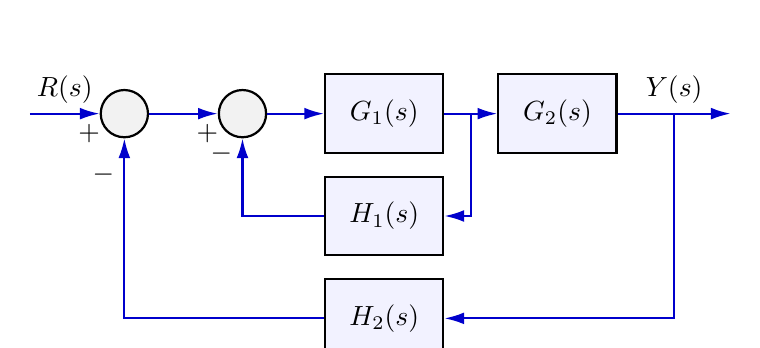
\begin{tikzpicture}[auto, node distance=2cm, >=Latex]
    \node [input, name=input] {};
    \node [sum, right of=input, node distance=1.2cm] (sum1) {};
    \node [sum, right of=sum1, node distance=1.5cm] (sum2) {};
    \node [block, right of=sum2, node distance=1.8cm] (g1) {$G_1(s)$};
    \node [block, right of=g1, node distance=2.2cm] (g2) {$G_2(s)$};
    \node [output, right of=g2, node distance=2.2cm] (output) {};
    
    \draw [sfgarrow] (input) -- node {$R(s)$} node[pos=0.85, below] {$+$} (sum1);
    \draw [sfgarrow] (sum1) -- node[pos=0.85, below] {$+$} (sum2);
    \draw [sfgarrow] (sum2) -- (g1);
    \draw [sfgarrow] (g1) -- (g2);
    \draw [sfgarrow] (g2) -- node [name=y] {$Y(s)$}(output);
    
    % Lup Umpan Balik Dalam H1
    \node [block, below of=g1, node distance=1.3cm] (h1) {$H_1(s)$};
    \draw [sfgarrow] ($(g1.east)!0.5!(g2.west)$) |- (h1);
    \draw [sfgarrow] (h1) -| node[pos=0.9, left] {$-$} (sum2);
    
    % Lup Umpan Balik Luar H2
    \node [block, below of=h1, node distance=1.3cm] (h2) {$H_2(s)$};
    \draw [sfgarrow] ($(g2.east)!0.5!(output)$) |- (h2);
    \draw [sfgarrow] (h2) -| node[pos=0.9, left] {$-$} (sum1);
\end{tikzpicture}
\end{center}
\begin{enumerate}[label=(\alph*)]
    \item Reduksi lup umpan balik bagian dalam yang melibatkan blok $G_1(s)$ dan $H_1(s)$.
    \item Tentukan fungsi transfer lingkar tertutup total $T(s) = \frac{Y(s)}{R(s)}$ menggunakan aljabar diagram blok.
\end{enumerate}

\textbf{Penyelesaian:}

\textbf{(a) Reduksi Lup Umpan Balik Bagian Dalam}

Perhatikan sub-sistem lingkar tertutup bagian dalam dengan masukan dari titik penjumlahan kedua dan keluaran setelah blok $G_1(s)$.
Fungsi transfer ekuivalen untuk lup bagian dalam dengan umpan balik negatif bernilai:
$$G_{in}(s) = \frac{G_1(s)}{1 + G_1(s) H_1(s)}$$

Dengan mengganti sub-sistem bagian dalam dengan blok tunggal $G_{in}(s)$, diagram blok menjadi hubungan kaskade (seri) antara $G_{in}(s)$ dan $G_2(s)$:
$$G_{fwd}(s) = G_{in}(s) \cdot G_2(s) = \frac{G_1(s) G_2(s)}{1 + G_1(s) H_1(s)}$$

\textbf{(b) Reduksi Lup Umpan Balik Luar dan Fungsi Transfer Total}

Sistem sekarang tersederhana menjadi satu lup umpan balik tunggal dengan jalur maju $G_{fwd}(s)$ dan jalur umpan balik negatif $H_2(s)$.
Fungsi transfer lingkar tertutup total dihitung menggunakan rumus dasar umpan balik:
$$T(s) = \frac{Y(s)}{R(s)} = \frac{G_{fwd}(s)}{1 + G_{fwd}(s) H_2(s)}$$

Substitusi ekspresi $G_{fwd}(s)$ menghasilkan:
$$T(s) = \frac{\frac{G_1(s) G_2(s)}{1 + G_1(s) H_1(s)}}{1 + \left( \frac{G_1(s) G_2(s)}{1 + G_1(s) H_1(s)} \right) H_2(s)}$$

Dengan mengalikan pembilang dan penyebut dengan suku $(1 + G_1(s) H_1(s))$, diperoleh fungsi transfer sistem yang telah tereduksi sempurna:
$$T(s) = \frac{Y(s)}{R(s)} = \frac{G_1(s) G_2(s)}{1 + G_1(s) H_1(s) + G_1(s) G_2(s) H_2(s)}$$

\vspace{12pt}
\hrule
\vspace{10pt}

% =========================================================================
% SOAL 10
% =========================================================================
\textbf{\large No. 10}

\textbf{Soal:}  
Diberikan diagram aliran sinyal (\textit{Signal Flow Graph}, SFG) sebagai berikut:
\begin{center}
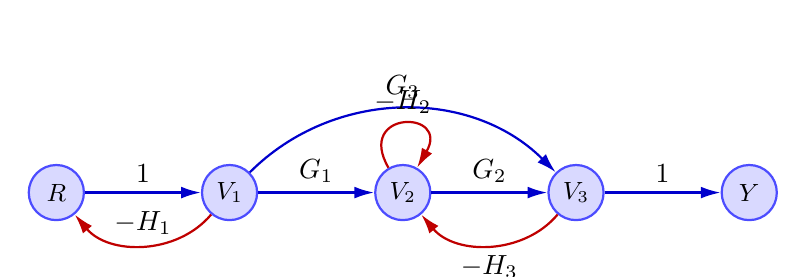
\begin{tikzpicture}[auto, node distance=2.2cm, >=Latex]
    \node [sfgnode] (R) {$R$};
    \node [sfgnode, right of=R] (V1) {$V_1$};
    \node [sfgnode, right of=V1] (V2) {$V_2$};
    \node [sfgnode, right of=V2] (V3) {$V_3$};
    \node [sfgnode, right of=V3] (Y) {$Y$};
    
    % Lintasan Maju Utama
    \draw [sfgarrow] (R) -- node {$1$} (V1);
    \draw [sfgarrow] (V1) -- node {$G_1$} (V2);
    \draw [sfgarrow] (V2) -- node {$G_2$} (V3);
    \draw [sfgarrow] (V3) -- node {$1$} (Y);
    
    % Lintasan Maju Bypass
    \draw [sfgarrow] (V1) to [bend left=45] node {$G_3$} (V3);
    
    % Loop Individual
    \draw [sfgloop] (V1) to [bend left=50] node [above] {$-H_1$} (R);
    \draw [sfgloop] (V2) to [out=120,in=60,looseness=6] node [above] {$-H_2$} (V2);
    \draw [sfgloop] (V3) to [bend left=50] node [below] {$-H_3$} (V2);
\end{tikzpicture}
\end{center}
\begin{enumerate}[label=(\alph*)]
    \item Tentukan seluruh lintasan maju (\textit{forward paths}) dan penguatannya ($P_k$).
    \item Tentukan seluruh loop tunggal (\textit{individual loop gains}) $L_i$.
    \item Tentukan pasangan loop yang tidak saling bersentuhan (\textit{non-touching loops}).
    \item Hitung determinan graf $\Delta$ dan kofaktor masing-masing lintasan $\Delta_k$.
    \item Tentukan fungsi transfer total $\frac{Y(s)}{R(s)}$ menggunakan Aturan Penguatan Mason (\textit{Mason's Gain Formula}).
\end{enumerate}

\textbf{Penyelesaian:}

\textbf{(a) Lintasan Maju (\textit{Forward Paths})}

Terdapat dua lintasan maju yang mengalirkan sinyal langsung dari node masukan $R$ ke node keluaran $Y$ tanpa mengunjungi satu simpul pun lebih dari satu kali:
$$P_1 = (1) \cdot G_1 \cdot G_2 \cdot (1) = G_1 G_2 \quad (\text{melalui node } R \to V_1 \to V_2 \to V_3 \to Y)$$
$$P_2 = (1) \cdot G_3 \cdot (1) = G_3 \quad (\text{melalui jalur pintas } R \to V_1 \to V_3 \to Y)$$

\textbf{(b) Loop Tunggal (\textit{Individual Loops})}

Ditemukan tiga loop umpan balik tertutup pada graf:
$$L_1 = 1 \cdot (-H_1) = -H_1 \quad (\text{loop antara node } R \text{ dan } V_1)$$
$$L_2 = -H_2 \quad (\text{self-loop pada node } V_2)$$
$$L_3 = G_2 \cdot (-H_3) = -G_2 H_3 \quad (\text{loop antara node } V_2 \text{ dan } V_3)$$

\textbf{(c) Pasangan Loop Non-Touching}

Pemeriksaan node-node yang dikunjungi oleh masing-masing loop:
- Loop $L_1$ melibatkan simpul $\{R, V_1\}$.
- Loop $L_2$ melibatkan simpul $\{V_2\}$.
- Loop $L_3$ melibatkan simpul $\{V_2, V_3\}$.

Karena loop $L_1$ dan loop $L_2$ tidak berbagi simpul yang sama ($\{R, V_1\} \cap \{V_2\} = \emptyset$), keduanya merupakan pasangan loop yang tidak bersentuhan:
$$L_1 L_2 = (-H_1)(-H_2) = H_1 H_2$$

Demikian pula, loop $L_1$ dan loop $L_3$ tidak berbagi simpul ($\{R, V_1\} \cap \{V_2, V_3\} = \emptyset$), sehingga membentuk pasangan kedua:
$$L_1 L_3 = (-H_1)(-G_2 H_3) = G_2 H_1 H_3$$

Loop $L_2$ dan $L_3$ bersentuhan di simpul $V_2$, dan tidak terdapat kombinasi tiga loop yang saling lepas secara simultan.

\textbf{(d) Determinan Graf dan Kofaktor Lintasan}

Determinan graf dihitung berdasarkan rumus Mason:
\begin{align*}
    \Delta &= 1 - (L_1 + L_2 + L_3) + (L_1 L_2 + L_1 L_3) \\
    &= 1 - (-H_1 - H_2 - G_2 H_3) + (H_1 H_2 + G_2 H_1 H_3) \\
    &= 1 + H_1 + H_2 + G_2 H_3 + H_1 H_2 + G_2 H_1 H_3
\end{align*}

Kofaktor lintasan dihitung dengan mengeliminasi loop yang bersentuhan dengan jalur maju:
- Lintasan $P_1$ melalui simpul $\{R, V_1, V_2, V_3, Y\}$, sehingga menyentuh seluruh ketiga loop. Akibatnya:
  $$\Delta_1 = 1$$
- Lintasan $P_2$ melalui simpul $\{R, V_1, V_3, Y\}$. Simpul $V_2$ tidak dilewati oleh lintasan $P_2$, sehingga loop $L_2$ tidak bersentuhan dengan lintasan $P_2$:
  $$\Delta_2 = 1 - L_2 = 1 - (-H_2) = 1 + H_2$$

\textbf{(e) Penentuan Fungsi Transfer Total via Aturan Mason}

Penerapan rumus penguatan Mason:
$$\frac{Y(s)}{R(s)} = \frac{P_1 \Delta_1 + P_2 \Delta_2}{\Delta} = \frac{G_1 G_2 (1) + G_3 (1 + H_2)}{1 + H_1 + H_2 + G_2 H_3 + H_1 H_2 + G_2 H_1 H_3}$$

\vspace{12pt}
\hrule
\vspace{10pt}

% =========================================================================
% SOAL 11
% =========================================================================
\textbf{\large No. 11}

\textbf{Soal:}  
Diberikan representasi multivariabel matematis:
\begin{enumerate}[label=(\alph*)]
    \item Suatu sistem satu-masukan dua-keluaran (SIMO) memiliki fungsi transfer:
    $$\mathbf{G}_{SIMO}(s) = \frac{1}{s^2 + 5s + 6} \begin{bmatrix} 2s + 1 \\ 3s + 4 \end{bmatrix}$$
    Tentukan representasi ruang keadaan dalam Bentuk Kanonik Keterkontrolan (CCF) bersama.
    \item Suatu sistem dua-masukan satu-keluaran (MISO) memiliki fungsi transfer:
    $$\mathbf{G}_{MISO}(s) = \frac{1}{s^2 + 4s + 3} \begin{bmatrix} s + 2 & 5 \end{bmatrix}$$
    Tentukan representasi ruang keadaan dalam Bentuk Kanonik Keterobservasian (OCF) bersama.
\end{enumerate}

\textbf{Penyelesaian:}

\textbf{(a) Konstruksi CCF Bersama untuk Sistem SIMO}

Karena kedua saluran keluaran memiliki polinomial penyebut bersama yang sama yaitu $d(s) = s^2 + 5s + 6$, diperkenalkan satu variabel perantara skalar $Z(s)$ untuk masukan tunggal $U(s)$:
$$Z(s) = \frac{U(s)}{s^2 + 5s + 6} \implies \ddot{z}(t) + 5\dot{z}(t) + 6z(t) = u(t)$$

Variabel-variabel keadaan didefinisikan sama seperti sistem skalar:
$$x_1(t) = z(t), \quad x_2(t) = \dot{z}(t)$$
$$\dot{x}_1(t) = x_2(t)$$
$$\dot{x}_2(t) = -6x_1(t) - 5x_2(t) + u(t)$$

Kedua sinyal keluaran dihubungkan secara langsung ke vektor keadaan melalui pembilangnya masing-masing:
$$Y_1(s) = (2s + 1) Z(s) = 1 Z(s) + 2 s Z(s) \implies y_1(t) = x_1(t) + 2x_2(t)$$
$$Y_2(s) = (3s + 4) Z(s) = 4 Z(s) + 3 s Z(s) \implies y_2(t) = 4x_1(t) + 3x_2(t)$$

Dalam representasi matriks:
$$A = \begin{bmatrix} 0 & 1 \\ -6 & -5 \end{bmatrix}, \quad B = \begin{bmatrix} 0 \\ 1 \end{bmatrix}$$
$$C = \begin{bmatrix} 1 & 2 \\ 4 & 3 \end{bmatrix}, \quad D = \begin{bmatrix} 0 \\ 0 \end{bmatrix}$$

\textbf{(b) Konstruksi OCF Bersama untuk Sistem MISO}

Untuk sistem MISO dengan satu keluaran dan dua masukan dengan penyebut $d(s) = s^2 + 4s + 3$, digunakan struktur OCF di mana matriks sistem $A$ dan vektor baris keluaran $C$ memiliki struktur standar skalar:
$$A = \begin{bmatrix} 0 & -3 \\ 1 & -4 \end{bmatrix}, \quad C = \begin{bmatrix} 0 & 1 \end{bmatrix}$$

Matriks masukan $B \in \mathbb{R}^{2 \times 2}$ disusun dari koefisien masing-masing pembilang masukan:
Untuk masukan pertama $U_1(s)$, pembilangnya adalah $s + 2 = 2 + 1s \implies B_1 = \begin{bmatrix} 2 \\ 1 \end{bmatrix}$.
Untuk masukan kedua $U_2(s)$, pembilangnya adalah $5 = 5 + 0s \implies B_2 = \begin{bmatrix} 5 \\ 0 \end{bmatrix}$.

Dengan menyatukan kedua kolom:
$$B = \begin{bmatrix} 2 & 5 \\ 1 & 0 \end{bmatrix}, \quad D = \begin{bmatrix} 0 & 0 \end{bmatrix}$$

Verifikasi dilakukan melalui perkalian matriks $C(sI - A)^{-1} B$:
$$(sI - A) = \begin{bmatrix} s & 3 \\ -1 & s+4 \end{bmatrix} \implies \operatorname{adj}(sI - A) = \begin{bmatrix} s+4 & -3 \\ 1 & s \end{bmatrix}$$
$$C \operatorname{adj}(sI - A) = \begin{bmatrix} 0 & 1 \end{bmatrix} \begin{bmatrix} s+4 & -3 \\ 1 & s \end{bmatrix} = \begin{bmatrix} 1 & s \end{bmatrix}$$
$$C \operatorname{adj}(sI - A) B = \begin{bmatrix} 1 & s \end{bmatrix} \begin{bmatrix} 2 & 5 \\ 1 & 0 \end{bmatrix} = \begin{bmatrix} 2 + s & 5 \end{bmatrix}$$
Hasil bagi dengan $\det(sI - A) = s^2 + 4s + 3$ menghasilkan fungsi transfer MISO yang identik.

\vspace{12pt}
\hrule
\vspace{10pt}

% =========================================================================
% SOAL 12
% =========================================================================
\textbf{\large No. 12}

\textbf{Soal:}  
Diberikan sistem ruang keadaan kontinu:
$$\dot{\mathbf{x}}(t) = \begin{bmatrix} 1 & 2 \\ 0 & 3 \end{bmatrix} \mathbf{x}(t) + \begin{bmatrix} 1 \\ 1 \end{bmatrix} u(t), \quad y(t) = \begin{bmatrix} 2 & 1 \end{bmatrix} \mathbf{x}(t)$$
\begin{enumerate}[label=(\alph*)]
    \item Tentukan nilai eigen dan matriks modal $P$ yang mendiagonalkan matriks $A$.
    \item Lakukan transformasi keserupaan (\textit{similarity transformation}) dengan koordinat baru $\mathbf{z}(t) = P^{-1}\mathbf{x}(t)$ untuk memperoleh representasi ruang keadaan baru $(\tilde{A}, \tilde{B}, \tilde{C}, \tilde{D})$.
    \item Buktikan bahwa fungsi transfer sistem bernilai invarian (tidak berubah) di bawah transformasi koordinat tersebut.
\end{enumerate}

\textbf{Penyelesaian:}

\textbf{(a) Nilai Eigen dan Matriks Modal}

Matriks $A$ merupakan matriks segitiga atas dengan nilai eigen diagonal:
$$\lambda_1 = 1, \quad \lambda_2 = 3$$

Vektor eigen untuk $\lambda_1 = 1$:
$$(A - I)\mathbf{v}_1 = \mathbf{0} \implies \begin{bmatrix} 0 & 2 \\ 0 & 2 \end{bmatrix} \begin{bmatrix} v_{11} \\ v_{21} \end{bmatrix} = \begin{bmatrix} 0 \\ 0 \end{bmatrix} \implies v_{21} = 0, \quad \mathbf{v}_1 = \begin{bmatrix} 1 \\ 0 \end{bmatrix}$$

Vektor eigen untuk $\lambda_2 = 3$:
$$(A - 3I)\mathbf{v}_2 = \mathbf{0} \implies \begin{bmatrix} -2 & 2 \\ 0 & 0 \end{bmatrix} \begin{bmatrix} v_{12} \\ v_{22} \end{bmatrix} = \begin{bmatrix} 0 \\ 0 \end{bmatrix} \implies -2v_{12} + 2v_{22} = 0 \implies \mathbf{v}_2 = \begin{bmatrix} 1 \\ 1 \end{bmatrix}$$

Matriks modal $P$ disusun dari kedua vektor eigen, dan inversnya dihitung:
$$P = \begin{bmatrix} 1 & 1 \\ 0 & 1 \end{bmatrix}, \quad P^{-1} = \begin{bmatrix} 1 & -1 \\ 0 & 1 \end{bmatrix}$$

\textbf{(b) Transformasi Keserupaan}

Matriks-matriks sistem baru dalam koordinat $\mathbf{z}(t)$ adalah:
$$\tilde{A} = P^{-1} A P = \begin{bmatrix} 1 & -1 \\ 0 & 1 \end{bmatrix} \begin{bmatrix} 1 & 2 \\ 0 & 3 \end{bmatrix} \begin{bmatrix} 1 & 1 \\ 0 & 1 \end{bmatrix} = \begin{bmatrix} 1 & 0 \\ 0 & 3 \end{bmatrix}$$
$$\tilde{B} = P^{-1} B = \begin{bmatrix} 1 & -1 \\ 0 & 1 \end{bmatrix} \begin{bmatrix} 1 \\ 1 \end{bmatrix} = \begin{bmatrix} 1 - 1 \\ 1 \end{bmatrix} = \begin{bmatrix} 0 \\ 1 \end{bmatrix}$$
$$\tilde{C} = C P = \begin{bmatrix} 2 & 1 \end{bmatrix} \begin{bmatrix} 1 & 1 \\ 0 & 1 \end{bmatrix} = \begin{bmatrix} 2 & 3 \end{bmatrix}, \quad \tilde{D} = D = 0$$

\textbf{(c) Pembuktian Invariansi Fungsi Transfer}

Fungsi transfer dari sistem asli $(A, B, C, D)$:
$$(sI - A)^{-1} = \begin{bmatrix} s-1 & -2 \\ 0 & s-3 \end{bmatrix}^{-1} = \frac{1}{(s-1)(s-3)} \begin{bmatrix} s-3 & 2 \\ 0 & s-1 \end{bmatrix}$$
$$(sI - A)^{-1} B = \frac{1}{(s-1)(s-3)} \begin{bmatrix} s-3 & 2 \\ 0 & s-1 \end{bmatrix} \begin{bmatrix} 1 \\ 1 \end{bmatrix} = \frac{1}{(s-1)(s-3)} \begin{bmatrix} s-1 \\ s-1 \end{bmatrix} = \begin{bmatrix} \frac{1}{s-3} \\ \frac{1}{s-3} \end{bmatrix}$$
$$G(s) = C (sI - A)^{-1} B = \begin{bmatrix} 2 & 1 \end{bmatrix} \begin{bmatrix} \frac{1}{s-3} \\ \frac{1}{s-3} \end{bmatrix} = \frac{2}{s-3} + \frac{1}{s-3} = \frac{3}{s-3}$$

Fungsi transfer dari sistem hasil transformasi $(\tilde{A}, \tilde{B}, \tilde{C}, \tilde{D})$:
$$\tilde{G}(s) = \tilde{C} (sI - \tilde{A})^{-1} \tilde{B} = \begin{bmatrix} 2 & 3 \end{bmatrix} \begin{bmatrix} \frac{1}{s-1} & 0 \\ 0 & \frac{1}{s-3} \end{bmatrix} \begin{bmatrix} 0 \\ 1 \end{bmatrix} = \begin{bmatrix} 2 & 3 \end{bmatrix} \begin{bmatrix} 0 \\ \frac{1}{s-3} \end{bmatrix} = \frac{3}{s-3}$$

Terbukti secara eksak bahwa:
$$\tilde{G}(s) \equiv G(s) = \frac{3}{s-3}$$
Fungsi transfer bersifat invarian terhadap transformasi keserupaan.

\end{document}
